\documentclass[slides]{pgnotes}

\title{Relational database management systems review}

\begin{document}

\maketitle

\tableofcontents

\section{Database management systems (DBMS)}\label{sec:dbms}

DataBase Management Systems (DBMS) \textit{persistently} store data \textbf{records} according to a \textbf{schema}.

\begin{bluebox}{Key concepts}
\begin{description}
\item[Schema] defines \textit{how} data is stored. Defines rules.
\item[Records] of logically grouped data (e.g. a customer, an invoice)
\end{description}
\end{bluebox}

\subsection{Required functionality}

\begin{greenbox}{Must provide}
\begin{description}
\item[Data storage/retrieval:] fundamental reason for using! 
\item[Catalog] of schema and data stored
\item[Transaction support] for batch updates to be applied atomically
\item[Concurrency control] to manage simultaneously connected clients
\item[Recovery] to a working state after hardware / software failures
\item[Authorization services] to verify connected clients identity and control access.
\item[Data communication support] to allow usage from remote computers.
\item[Integrity services] to enforce constraints on data as defined by the user.
\end{description}
\end{greenbox}

\subsection{Families}

\begin{greenbox}{Relational databases}
  \begin{itemize}
  \item Sometimes called \textbf{SQL databases}.
  \item Examples: Oracle, PostgreSQL, MySQL, Microsoft SQL.
  \end{itemize}
\end{greenbox}

\begin{bluebox}{Non-relational databases}
  \begin{description}
  \item[Key-Value stores] that associate a key with a value. (e.g. Redis)
    \begin{itemize}
    \item Optimised for fast lookup of small pieces of data
    \end{itemize}
  \item[Document databases] that store a semi-structured document identified by a key (e.g. MongoDB)
    \begin{itemize}
    \item Useful for semi-structured data accessed as a whole
    \end{itemize}
  \item[Graph databases] that store nodes and their relationships (e.g. Neo4J)
    \begin{itemize}
    \item Mapping, transport planning, relationships, likes, friends.
    \end{itemize}
  \end{description}
\end{bluebox}

We'll recap \textbf{relational databases} using \textbf{PostgreSQL}.

\subsection{PostgreSQL}\label{sec:postgresql}

We will focus on PostgreSQL as our primary relational database.


\begin{greenbox}{Reasons for choice of PostgreSQL:}
\begin{itemize}
\item
  It is free software
\item
  Can be installed on many operating systems.
\item
  No limits / free-trial limitations.
\item
  Support exists for geospatial data, JSON, XML, full-text search etc.
\item
  Has some support for masquerading as other types of DB (e.g. graph data).
\item
  High adoption among many analytics and data science workloads.
\end{itemize}
\end{greenbox}

As we continue we will refer to PostgreSQL as \textbf{Postgres} for brevity.

On a single host, a relational database management system \textbf{cluster} provides one or more isolated \textbf{databases}.
Within a database, data is contained in one or more \textbf{tables} according to the \textbf{schema}.


\subsection{Text-based query language}

DBMS normally incorporate a native programming language allowing us either directly or via a client application manipulate the database: 

\begin{greenbox}{3 roles:}
\begin{description}
\item[Data Definition (DDL)] to work with schema.
\item[Data Manipulation (DML)] to work with data stored according to the schema.
\item[Query language] for accessing data (part of DML)
\end{description}
\end{greenbox}

Usually a common language provides all of these functions.
SQL best known and most commonly employed:

\begin{minted}{sql}
  SELECT name, finish_time
  FROM competitors
  ORDER BY finish_time DESC;
\end{minted}

\subsection{Database host}

The server process manages the data store and processes requests from clients.
The server can be running on any of the following \emph{hosts}:

\begin{greenbox}{Hosts}
  \begin{itemize}
  \item
    Standard laptop / desktop computer
  \item
    Dedicated server computer (in a data centre environment)
  \item
    Cloud-based virtual host, called a compute instance. (e.g.~Amazon EC2)
  \item
    A managed database service provided by a cloud service provider
    (e.g.~Amazon RDS, Azure, Google Cloud, IBM Cloud)
  \end{itemize}
\end{greenbox}

Database is often a critical piece of our infrastructure and needs to be provisioned appropriately. \textit{Will discuss data centre environment later on!}

DBMS can run on a variety of Operating Systems (often UNIX / Linux).


\subsection{Client-server}\label{client-server}

Most database management systems run in a client-server model, even on the same host.

\begin{figure}[htbp]
  \centering
  \includegraphics[width=0.7\linewidth]{dbms_client_server}
  \caption{Client-Server model}
  \label{fig:client-server-model}
\end{figure}


\subsection{Protocol}

The client program accesses the server using a server-specific \textbf{protocol}.

Clients normally access the server through IP networks using TCP on a specified port number.

\begin{greenbox}{Examples of clients}
\begin{itemize}
\item
  Most databases have a simple command-line client that can send
  requests to the database and display results
\item
  Programs / apps / scripts can be written to access database servers using a client library.
  \begin{itemize}
  \item
    Generally the bundled text-mode client uses this library internally too!
  \end{itemize}
\end{itemize}
\end{greenbox}

\begin{redbox}{Important note about clients / servers}
\begin{itemize}
\item
  The client may in some cases be running on the same host as the
  server.
\item
  Software that is the client of a DBMS may itself be a server of another type.
\end{itemize}
\end{redbox}



\subsection{Concurrency}
\label{sec:concurrency}

This also implies that there is a degree of concurrency, where multiple
clients access the same database at the same time.

\begin{figure}[htbp]
  \centering
  \includegraphics[width=1.0\linewidth]{dbms_concurrent_access}
  \caption{Concurrent access to a college timetable database}
  \label{fig:concurrent-access}
\end{figure}

Clients are often heterogeneous, where different types of clients concurrently access the same data.



\subsection{Remote access}

A particular pattern you will encounter is where the client program runs on the same host as the DBMS, and remote shell access is used to permit clients to connect to the server.

\begin{figure}[htbp]
  \centering
  \includegraphics[width=1.0\linewidth]{ssh_psql_usage}
  \caption{SSH access to a remote database}
  \label{fig:ssh-psql-usage}
\end{figure}





\section{Relational databases (RDBMS)}\label{sec:relational-databases}

Codd's Seminal paper defines a set of characteristics that a relational database must possess.

We'll use these to explore the basic anatomy of a relational database, specifically PostgreSQL.

Note: the order of these rules has been adjusted to introduce some concepts in a more logical way!


\subsection{Foundation rule}

\textbf{For any system that is advertised as, or claimed to be, a relational database management system, that system must be able to manage databases entirely through its relational capabilities.}
  
\subsection{Information Rule}
  
\textbf{All information in a relational database is represented explicitly at the logical level and in exactly one way --- by values in tables.}

\subsubsection{Relational data structure}

\begin{figure}[htbp]
  \centering
  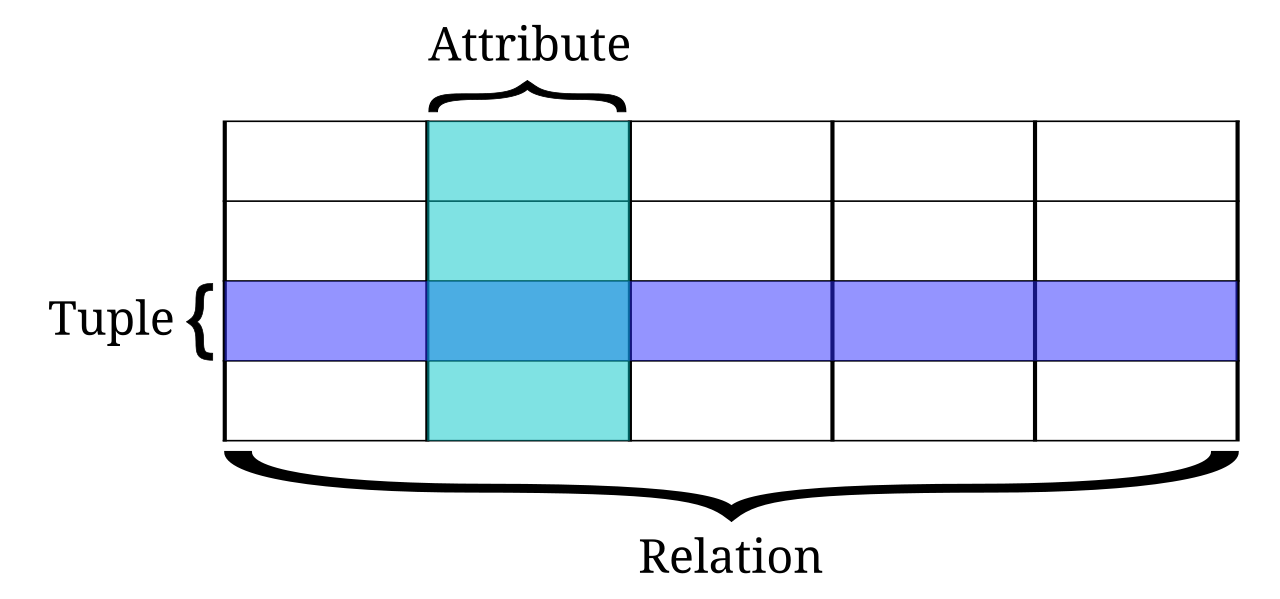
\includegraphics[width=0.5\linewidth]{rdbms_terms}
  \caption{Relational model terminology}
  \label{fig:rdbms-terms}
\end{figure}

\begin{description}
\item[Relation (Table):] with columns and rows. Table names must be unique.
  \begin{description}
  \item[Base relation] is a table defined in the database schema
  \item[Derived relation] is a virtual table that appears in response to a query
  \end{description}
\item[Attribute (Column):] holding distinct part of a row: 
  \begin{itemize}
  \item Column names must be unique within a table.
  \item Column has a \textbf{data type} (e.g. integer, text) from an allowable list (database-dependent).
  \item Column may allow / permit \textbf{null} values (unknown, empty, undefined, blank)
  \item Column order has no meaning or significance.
  \end{itemize}
\item[Tuple (Row):] a single record contained with a table.
  \begin{itemize}
  \item No theoretical upper limit on number of rows.
  \item The natural order of rows in a table is meaningless!  Do not rely on it!
  \end{itemize}
\end{description}

\subsection{Systematic treatment of null values}
  \textbf{Null values (distinct from the empty character string or a string of blank characters and distinct from zero or any other number) are supported in fully relational DBMS for representing missing information and inapplicable information in a systematic way, independent of data type.}

\subsubsection{Null}

Null denotes a lack of a value, used to indicate that data is missing, unknown, blank, undefined:
\begin{itemize}
\item Null is \textbf{not} zero, the empty string, false or any other value.
\item Null values will \textbf{pollute other expressions} (e.g. arithmetic, comparison)
  \begin{itemize}
  \item Null does not even equal null!
  \end{itemize}
\item \textbf{Can test} for null with \texttt{IS NULL} operation.
\end{itemize}
While the concept of null can be confusing, it avoids placeholder data.



\subsection{Integrity independence}

\textbf{Integrity constraints specific to a particular relational database must be definable in the relational data sublanguage and storable in the catalog, not in the application programs.}

\subsubsection{Unique constraint}

Within a table, a unique constraint on a column or group of columns will prevent duplicate rows existing.  

\newpage

\subsubsection{Primary key}

Practically we need ways to identify any row individually.
Within any table, there may be a number of \textbf{candidate keys} that could be used to identify each row.
\begin{description}
\item[Simple key:] a single column that is:
  \begin{description}
  \item[not null] so that every row can be identified.
  \item[unique] so that every row is distinct. 
  \end{description}
\item[Complex key:] two or more columns:
  \begin{enumerate}
  \item no columns in the key are null
  \item together are unique
  \end{enumerate}
\end{description}
For each table, one of its candidate keys is selected as the \textbf{primary key}.

Should always be encoded explicitly by DML in the database.


\subsection{Guaranteed access rule}

\textbf{Each and every datum (atomic value) in a relational database is guaranteed to be logically accessible by resorting to a combination of table name, primary key value and column name.}

\begin{description}
\item Often in practice we are operating on groups of rows where we select them based on the values of one or more columns. 
\end{description}
  


\subsection{Comprehensive data sublanguage rule}

A relational system may support several languages ... However, there must be at least one language whose statements are expressible, per some well-defined syntax, as character strings and that is comprehensive in supporting all of the following items:

\begin{enumerate}
\item Data definition.
\item View definition.
\item Data manipulation (interactive and by program).
\item Integrity constraints.
\item Authorization.
\item Transaction boundaries (begin, commit and rollback). \textit{We will meet transactions again later on.}
\end{enumerate}

\textbf{In PostgreSQL's case, its adoption of SQL fits this rule.}


  
\subsection{Dynamic online catalog based on the relational model}

\textbf{The database description is represented at the logical level in the same way as ordinary data, so that authorized users can apply the same relational language to its interrogation as they apply to the regular data.}

\begin{greenbox}{In practical terms}
  The DBMS can provide the schema for any table using the same methods we'd use to query data.
  \begin{itemize}
  \item Self-documenting 
  \item Output can be used for generating reports, diagrams etc.
  \end{itemize}
\end{greenbox}


\subsection{View updating rule}
  All views that are theoretically updatable are also updatable by the system.

  \begin{greenbox}{Practical meaning}
    \begin{itemize}
    \item Relational databases can have views made up of data dynamically drawn on demand from different tables, but should appear as a single table.
    \item In theory these should be updateable but in practice we have to tell the DB how to do it.
    \item \textit{We'll come back to this one later when you're familiar with views.}
    \end{itemize}
  \end{greenbox}
  
\subsection{Relational Operations Rule / Possible for high-level insert, update, and delete}
  The capability of handling a base relation or a derived relation as a single operand applies not only to the retrieval of data but also to the insertion, update and deletion of data.

\subsection{Physical data independence}
  Application programs and terminal activities remain logically unimpaired whenever any changes are made in either storage representations or access methods.

  \begin{greenbox}{Practical meaning}
    \begin{itemize}
    \item Changes made to the database software in how it internally stores data shouldn't be visible or require any changes at the client level.
    \end{itemize}
  \end{greenbox}
  
\subsection{Logical data independence}
Application programs and terminal activities remain logically unimpaired when information-preserving changes of any kind that theoretically permit unimpairment are made to the base tables.

\begin{greenbox}{Practical meaning}
  \begin{itemize}
  \item Changes made in the database structure shouldn't affect programs accessing it.
  \item Difficult to practically achieve in practice!
  \end{itemize}
\end{greenbox}

  
\subsection{Distribution independence}
The end-user must not be able to see that the data is distributed over various locations. Users should always get the impression that the data is located at one site only.

\begin{greenbox}{Practical meaning}
\begin{itemize}
\item  We shouldn't be concerned that the DBMS is storing data on multiple file(s) on disk(s).
\item  More complex DBMS installations may be distributing or \textit{sharding} data over different nodes for space scalability. 
\end{itemize}
\end{greenbox}


\subsection{Non-subversion rule}
  If a relational system has a low-level (single-record-at-a-time) language, that low level cannot be used to subvert or bypass the integrity rules and constraints expressed in the higher level relational language (multiple-records-at-a-time).

  \begin{greenbox}{Practical meaning}
   There can't be a ``bypass'' switch on the integrity constraints!
  \end{greenbox}

\section{Single-table databases}

Recall that:

\begin{itemize}
\item A PostgreSQL \textit{cluster} provides:
\item One or more \textbf{databases} that each have
\item (One or more \textbf{schemas} that each hold)
\item One or more \textbf{tables}
\end{itemize}

where each table:

\begin{itemize}
\item has separate \textbf{columns} holding individual attribute values
\item stores data each record in \textbf{rows}
\end{itemize}


\subsection{Data definition language}

Key concepts will be easily learned through repeated practice and
reference to

\begin{description}
\item[CREATE table]
  to define table name, columns (type, constraints)
\item[ALTER table]
  for incremental changes.
\item[DROP table]
  without warning!
\end{description}

Sometimes it's easiest to specify information up front in the \texttt{CREATE} statement.

Often it's better to start with a workable definition and amend using\texttt{ALTER}.

\subsection{Sample problem}

We will mainly do this by example.

\begin{greenbox}{Example}
  Mary is a local crafter who makes her own pottery.
  She runs a small shop where she sells her own wares.

  At the moment she writes down all sales in a book:
  \begin{itemize}
  \item Date and sometimes time
  \item Description of what sold
  \item Quantity
  \item Price
  \item Total
  \end{itemize}

  Having done a database class, she realises that she could easily put together a table to replace the book.
\end{greenbox}

\subsection{Table names}

Following a consistent and workable pattern with table names will help a lot:

\begin{enumerate}
\item names should be \textbf{descriptive}
  \begin{itemize}
  \item decide on a sensible structure on pluralisation
  \end{itemize}
\item try to keep names reasonablly \textbf{short}
  \begin{itemize}
  \item You will be typing them a lot!
  \end{itemize}
\item do not use spaces, use the underscore instead (\_)
  \begin{itemize}
  \item spaces in most text-based systems are a receipe for disaster!
  \end{itemize}
\item table names are \textbf{case insensitive}
\end{enumerate}

Table names \textit{can} be changed afterwards.

Our table will be called \textbf{sales}.


\subsection{Column names}

Similar set of rules for columns as for tables:

Again following a consistent and workable pattern with column names will help a lot:

\begin{enumerate}
\item names should be \textbf{descriptive}
\item try to keep names reasonablly \textbf{short}
\item do not use spaces, use the underscore instead (\_)
\end{enumerate}

Column names \textit{can} be changed afterwards.

\newpage

\begin{greenbox}{Example}

  In our example, we'll choose the following column names:

  \begin{enumerate}
  \item \texttt{timestamp}
  \item \texttt{description}
  \item \texttt{quantity}
  \item \texttt{total\_price}
  \end{enumerate}

\end{greenbox}

\section{Datatypes and constraints} 

\textbf{Choosing the correct datatypes is vitally important for making a usable database!}

\begin{description}
\item[TEXT] for text (only!)
  \begin{itemize}
  \item Other database systems use CHAR, VARCHAR etc. Avoid!
  \end{itemize}
\item Numeric data largely falls into the categories of: integer, fixed precision and arbitary precision data.
  \begin{description}
  \item[INT] for integers
    \begin{itemize}
    \item Also have \texttt{SMALLINT, BIGINT} etc for range
    \end{itemize}
  \item[NUMERIC] for numeric data incl. decimals and currency
    \begin{itemize}
    \item Easy to make mistakes choosing float instead!
    \end{itemize}
  \end{description}
\end{description}

\subsection{Good practices}

\begin{enumerate}
  
\item Do not store numbers as text.

\item Do not store boolean true / false ( or any synonyms ) as text.

\item Do not sure enumerated types as text. Either use an ENUM and/or a foreign-keyed table.

\item Anything where you need absolute precision after the decimal point must be NUMERIC, not FLOAT. 
  
\item Do not be tempted to store a single logical date/time as separate date and time columns.
  Always use a single timestamp for this. 
  
\end{enumerate}


\subsection{NOT NULL}\label{not-null}

The NOT NULL constraint prevents a particular column value being null.
Writes will fail if set to NULL or if unspecified unless default column value specified.

\begin{verbatim}
-- During table creation:
CREATE TABLE tasks (
   description text not null,
   /* other columns */
);
\end{verbatim}

\newpage
\subsubsection{Changing NOT NULL status}

Whether NULL should be allowed depends on problem of interest.
By default NULL is allowed.
Must specify NOT NULL if not.

Can modify the column's NULLable status afterwards:
\begin{verbatim}
-- make a column NOT NULL
ALTER TABLE tasks ALTER COLUMN description SET NOT NULL

-- remove the NOT NULL constraint from a column
ALTER TABLE tasks ALTER COLUMN description DROP NOT NULL
\end{verbatim}

\begin{greenbox}{Example}
  In our example we will set all columns to not null, as none are optional.
\end{greenbox}


\subsection{UNIQUE}\label{unique}

The UNIQUE constraint prohibits two rows from having an equal set of
attribute values for the columns specified:

\begin{itemize}
\item Use UNIQUE after column definition if column should be unique
\item Use UNIQUE(col1, col2) if two or more columns should be unique after the column definitions
\end{itemize}

\newpage

\begin{verbatim}
-- During table creation:
CREATE TABLE tasks (
   description text unique,
   /* other columns as necessary */
   project_code text,
   subproject_code text,
   unique(project,subproject)
); 
\end{verbatim}

\begin{greenbox}{Example}
  In our example we've no UNIQUE columns (yet!)
\end{greenbox}

\newpage
\subsubsection{Modifying UNIQUE afterwards}

Just as with NOT NULL we can modify UNIQUE later on:

\begin{verbatim}
-- Afterwards
ALTER TABLE tasks ADD UNIQUE (project, subproject);
\end{verbatim}


\subsection{Default values}
\label{sec:default-values}

Default values are automatically inserted when unspecified in INSERT
statement.
Often used in conjunction with NOT NULL.
Can be static value or based on functions (see later).

\begin{verbatim}
-- when creating a table
CREATE TABLE sales (
    /* other columns  */
    quantity smallint not null default 1;
    timestamp timestamp not null default now(); 
);
\end{verbatim}


\newpage
\subsubsection{Altering DEFAULT}

\begin{verbatim}
-- afterwards
ALTER TABLE tasks ALTER COLUMN description SET default 'xyz'
ALTER TABLE tasks ALTER COLUMN description DROP default
\end{verbatim}


\section{Primary key}
\label{sec:primary-key}

\textbf{Primary key} value is a \textbf{unique} AND \textbf{not null}.

Unambiguously identifies each row.

Every table should have 1 primary key.
Cannot have more than 1. 

Most DBMS do not enforce this, but you should consider it mandatory.
Use PRIMARY KEY if column is the primary key. 

\begin{greenbox}{Example}
  In our example, we \textit{could} use the timestamp as the primary key.

  But it would be much better to make an autoincrementing integer \texttt{id} column.
\end{greenbox}

\newpage

\begin{verbatim}
-- specifying primary key
CREATE TABLE accounts ( 
    account_number bigint primary key
    /* other columns as necessary */
);

-- primary key covering two columns
CREATE TABLE accounts (
    branch bigint, -- not null automatic
    account_number bigint,  -- not null automatic
    /* other columns */
    primary key (branch, account_number)
    /* other constraints etc. */
)
\end{verbatim}

\subsection{Auto-increment column}
\label{sec:auto-increment-column}

We can use the column types SERIAL or BIGSERIAL for auto-incrementing columns.
Generally prefer SERIAL or BIGSERIAL.

Shorthand for default value based on \textit{sequence generator} (later on).

\begin{verbatim}
CREATE TABLE sales ( 
    id BIGSERIAL PRIMARY KEY,
    /* other columns & constraints */
);
\end{verbatim}


\subsection{DML operations}

The main \textbf{Data Manipulation Language} operations you'll use are grouped into:

\begin{description}
\item[INSERT]
  rows populating specified columns with data given.
\item[UPDATE]
  table, optionally select rows with \texttt{WHERE}.
\item[DELETE]
  rows from a table, optionally select rows with \texttt{WHERE}.
\end{description}

We'll mainly cover these by example!


\section{Transaction control}
\label{sec:transaction-control}

\href{https://www.postgresql.org/docs/15/tutorial-transactions.html}{PostgreSQL
transaction control} can be used in simplest form to give basic ``undo''
capability:

\begin{verbatim}
-- start a new transaction
BEGIN;

/* execute SQL statements then either: */

COMMIT; /* save the changes */
-- or
ROLLBACK; /* undo the changes */
\end{verbatim}

\subsection{Error handling}
\label{sec:error-handling}

If we don't BEGIN a transaction we implicitly BEGIN before the statement
and COMMIT after it. Errors (e.g.~syntax) will abort the transaction,
requiring a ROLLBACK before any more statements will be accepted.

\subsection{Savepoints}\label{savepoints}

\begin{verbatim}
BEGIN;

/* sql statement block 1 */

-- define a savepoint
SAVEPOINT sp1;

/* sql statement block 2 */

-- rollback to the savepoint undoes block 2; 
ROLLBACK TO sp1;

-- then either:
COMMIT; /* or ROLLBACK */
\end{verbatim}





\section{Multi-table databases}

\subsection{Scenario}

A group of local artisan producers operate a popup stall for a 3-month period.
They contract a local IT expert to build a simple sales tracking and reporting system.

\begin{bluebox}{Main requirements}
  \begin{enumerate}
  \item Sales must be numbered and timestamped.
  \item Every sale is separate (no concept of a ``basket'' for simplicity!)
  \item Stall accepts cash and card tender.
    \begin{itemize}
    \item Card payments have a 1.68\% processor fee (which may vary).
    \item May be requirement to accept additional payment types during period.
    \end{itemize}
  \item Sale must capture producer, description, quantity sold, amount paid and tender.
  \item Everyone will be paid at the end of the 3-month period.
  \item Database must be able to produce the following reports:
  \end{enumerate}
\end{bluebox}


\subsection{Implementation with 3 tables}

\begin{center}
\includegraphics[width=0.6\linewidth]{scenario}
\end{center}

\subsection{Key decisions}

\begin{enumerate}
\item \textbf{Auto-numbered} \texttt{id} column using \texttt{SERIAL}.
\item \textbf{Primary key} will be the auto-numbered \texttt{id} column.
\item All fields will be \textbf{not null}.
\item Every sale must match a valid:
  \begin{description}
  \item[producer] from the \texttt{producer} table.
  \item[tender] from the \texttt{tender} table.
  \end{description}
\item Storage of numerical values:
  \begin{description}
  \item[Amounts] as \texttt{NUMERIC(6,2)} typed \texttt{amount}.
  \item[Rate] as \texttt{NUMERIC(6,2)} typed \texttt{rate}. 
  \end{description}
\end{enumerate}

\section{Domains}\label{sec:domains}

\href{https://www.postgresql.org/docs/13/domains.html}{Domains} are
user-defined types based on underlying type. Defaults to NULL allowed,
best to define any NOT NULL conditions on the underlying columns. CHECK
constraints can be defined.

\begin{minted}{postgresql}
/* Number to hold 1-10 user rating */
CREATE DOMAIN rating AS integer CHECK ( VALUE >= 1 AND VALUE <=10 );

/* Just use the domain as type when creating table */
CREATE TABLE restaurants (
    id bigserial primary key,
    /* creating two columns using our domain: */
    visitor_rating rating not null,
    reviewer_rating rating, 
    /* other columns */
);
\end{minted}



\section{Foreign keys}\label{foreign-keys}

\href{https://www.postgresql.org/docs/13/ddl-constraints.html\#DDL-CONSTRAINTS-FK}{Foreign
keys} require that values in a column (or a group of columns) must match
the values appearing in some row of another table. This maintains the
referential integrity.

\begin{minted}{postgresql}
/* each employee must be in a valid department */

CREATE TABLE department (
id bigserial primary key,
name text not null unique
/* other fields as required */
);

CREATE TABLE employee (
id bigserial primary key,
surname text not null,
firstname text not null,
department bigint not null REFERENCES department
/* other fields as required */
)
\end{minted}

\subsection{DELETE / UPDATE behaviour}\label{delete-update-behaviour}

Possible behaviours: NO ACTION, CASCADE, SET NULL.

\begin{minted}{postgresql}
CREATE TABLE product ( 
/* other fields */

department bigint references departments, 
/* NO ACTION is the default, prohibits conflicting delete */

supplier bigint references suppliers ON DELETE CASCADE,
/* DELETE in suppliers deletes linked products */

policy bigint references policies ON DELETE SET NULL,
/* SETS product.policy to NULL when row in policies deleted  */

);
\end{minted}

\subsection{JOIN}\label{join}

The JOIN operation permits queries across more than one table. See both
the
\href{https://www.postgresql.org/docs/current/tutorial-join.html}{JOIN
tutorial} and the
\href{https://www.postgresql.org/docs/13/queries-table-expressions.html}{Table
expressions} section from Postgres manual for full details.

Assume R1 to be a row of Table T1. Similarly R2 for T2. Normally should
explicitly specify columns required and use table prefix to avoid
ambiguity.

\subsection{INNER JOIN}\label{inner-join}

For each row R1 of T1, the joined table has a row for each row in T2
that satisfies the join condition with R1.

\subsection{LEFT JOIN}\label{left-join}

Same as INNER JOIN except that output also includes any row in T1 that
does not match one or more rows in T2. Null values are substituted for
T2 in the output row.

\subsection{RIGHT JOIN}\label{right-join}

Similar to LEFT JOIN. Same as INNER JOIN, except any row in T2 that does
not match \(\ge 1\) rows in T1 will be output. Null values are
subtituted for T1 columns in the otuput row.

\subsection{FULL JOIN}\label{full-join}

Similar to combination of LEFT and RIGHT JOIN. INNER JOIN performed.
Then rows in T1 without corresponding T2 output with nulls for T2. Same
again, rows in T2 without corresponding T1 rows output with nulls for
T1.


\section{Views}\label{sec:views}

\href{https://www.postgresql.org/docs/13/tutorial-views.html}{Views} are
defined by @connolly:2015:database as:

\begin{quote}
The dynamic result of one or more relational operations operating on the
base relations to produce another relation. A view is a virtual relation
that does not necessarily exist in the database but can be produced upon
request by a particular user, at the time of the request.
\end{quote}

\begin{minted}{postgresql}
/* Creation syntax: */
CREATE VIEW my_view AS
SELECT ... ;
/* select statement can be any valid select */

/* VIEW can be selected like any other table */
SELECT * FROM my_view ; 
\end{minted}




\end{document}
